\documentclass[a4paper,12pt,twoside]{report}

\usepackage[utf8]{inputenc}    
\usepackage[T1]{fontenc}
\usepackage[french]{babel}  % Le dernier est pris en compte et \selectlanguage{} signifie que l'on passe à un autre langage
\usepackage[top=3.5cm, bottom=3.5cm, left=3.5cm, right=3.5cm]{geometry}
\usepackage{amsthm}
\usepackage{amsmath}
\usepackage{amssymb}
%\usepackage{mathrsfs}
\usepackage{dsfont}
\usepackage{empheq}
%\usepackage{isomath}
\usepackage{pstricks,pst-plot,pst-text,pst-tree,pst-eps,pst-fill,pst-node,pst-math,pstricks-add}
%\usepackage[charter]{mathdesign}
\usepackage{fourier}
\usepackage{helvet}
\usepackage{courier}
\usepackage[mathscr]{euscript}
\frenchbsetup{StandardLists=true} % Ã  inclure si on utilise \usepackage[french]{babel}
\usepackage{enumitem}
\usepackage{marvosym}
\usepackage{blkarray}
\usepackage{stmaryrd}
%\usepackage{pifont}
\usepackage{fancyhdr}
\usepackage{titletoc}
\usepackage[newparttoc]{titlesec}
\usepackage{titlesec}
\usepackage{xcolor}
%\usepackage{yhmath}
\usepackage{setspace}
\usepackage{color}
\usepackage[french]{minitoc}
\usepackage[most]{tcolorbox}
\usepackage{chngcntr}
\usepackage{graphicx}
\usepackage{float}
\usepackage{tikz,pgf}
\usetikzlibrary{arrows}
\usepackage{parskip}
\usepackage{makeidx}
%\usepackage{cleveref}
\usepackage{stackengine}
\usepackage{esvect}
\usepackage{hyperref}
\usepackage{listings}
\usepackage{caption}
\usepackage{subcaption}


\setlength{\parskip}{0.1cm}


\newcommand{\bigzero}{\mbox{\normalfont\Large\bfseries 0}}
\newcommand{\rvline}{\hspace*{-\arraycolsep}\vline\hspace*{-\arraycolsep}}
\newcommand{\hsp}{\hspace{20pt}}
\newcommand{\HRule}{\rule{\linewidth}{0.5mm}}

\setcounter{tocdepth}{2}
\setcounter{secnumdepth}{3}

% Lettres doubles
\newcommand{\R}{\mathbb{R}}
\newcommand{\K}{\mathbb{K}}
\newcommand{\A}{\mathbb{A}}
\newcommand{\F}{\mathbb{F}}
\newcommand{\C}{\mathbb{C}}
\newcommand{\N}{\mathbb{N}}
\newcommand{\E}{\mathbb{E}}
\newcommand{\Q}{\mathbb{Q}}
\newcommand{\Z}{\mathbb{Z}}
\newcommand{\1}{\mathbb{1}}
\newcommand{\T}{\mathbb{T}}
\renewcommand{\P}{\mathbb{P}}
\newcommand{\V}{\mathbb{V}}

\newcommand{\rot}{\mathrm{rot}\,}
% Complexes
\newcommand{\complex}{\mathrm{i}}
\newcommand{\complexj}{\mathrm{j}}
\newcommand{\partieRe}{\Re \mathrm{e}}
\newcommand{\partieIm}{\Im \mathrm{m}}

\renewcommand{\exp}{\mathrm{e}}
\newcommand{\diam}{\mathrm{diam}}
\newcommand{\dist}{\mathrm{dist}}


\newcommand{\Card}{\mathrm{Card}}
\newcommand{\permuS}{\mathfrak{S}}
\newcommand{\et}{\ \hbox{et}\ }
\newcommand{\ou}{\ \hbox{ou}\ }
\newcommand{\non}{\ \hbox{Non}\ }
\newcommand{\PGCD}{\mathrm{PGCD}\,}
\newcommand{\PPCM}{\mathrm{PPCM}\,}
\newcommand{\ie}{\emph{ie.}\text{ }}
\newcommand{\cf}{\emph{cf}\text{ }}
\newcommand{\la}{\left\langle}
\newcommand{\ra}{\right\rangle}

% Algèbre linéaire
\newcommand{\Mat}{\mathrm{Mat}}
\newcommand{\Id}{\mathrm{Id}}
\newcommand{\Vect}{\mathrm{Vect\,}}
\newcommand{\Ker}{\mathrm{ker\,}}
\newcommand{\tr}{\mathrm{Tr}\,}
\newcommand{\trace}{\mathrm{Tr\,}}
\newcommand{\im}{\mathrm{Im}\,}
\newcommand{\rg}{\mathrm{rg\, }}
\newcommand{\GL}{\mathrm{GL}}
\newcommand{\SL}{\mathrm{SL}}
\newcommand{\codim}{\mathrm{codim}}
\newcommand{\spec}{\mathrm{Spec}}
\newcommand{\trans}[1]{{\vphantom{#1}}^t \! #1}
\newcommand{\e}{\texttt{\textbf{e}}}
\newcommand{\f}{\texttt{\textbf{f}}}
\newcommand{\g}{\texttt{\textbf{g}}}
\newcommand{\nor}[1]{\left\Arrowvert #1 \right\Arrowvert}
\renewcommand{\div}{\mathrm{div}\,}

% Intégration
\renewcommand{\d}{\,\mathrm{d}}
\newcommand{\dx}{\, \mathrm{d}x}
\newcommand{\dy}{\, \mathrm{d}y}
\newcommand{\du}{\, \mathrm{d}u}
\newcommand{\dv}{\, \mathrm{d}v}
\newcommand{\ds}{\, \mathrm{d}s}
\newcommand{\dt}{\, \mathrm{d}t}
\newcommand{\dr}{\, \mathrm{d}r}

% Trigonométrie
\newcommand{\argch}{\mathrm{Argch}\; }
\newcommand{\argsh}{\mathrm{Argsh}\; }
\newcommand{\argth}{\mathrm{Argth}\; }

\newcommand{\sgn}{\mathrm{sgn}\,}
\newcommand{\proj}{\mathrm{proj}\,}


\newcommand{\contradiction}{\,\text{\Lightning}\,}
\newcommand{\annotation}[1]{
	\begin{center}
		{\small\itshape #1}
	\end{center}
}

\renewcommand{\Re}{\frak{R}\mathrm{e}\,}
\renewcommand{\Im}{\frak{I}\mathrm{m}\,}
\newcommand{\loc}{\mathrm{loc}}

\newcommand{\pagedegarde}[2]{\begin{titlepage}
		%\begin{sffamily}
		%\includegraphics[scale=0.2]{/home/matthieu/Documents/logo_bdx.jpg}~\\[2cm]
		\begin{center}
			
			% Upper part of the page. The '~' is needed because \\
			% only works if a paragraph has started.
			
			
			\LARGE Université de Bordeaux\\[2cm]
			
			\Large Master 1 : EDP - Modélisation - Probabilités\\[3cm]
			
			%\vfill
			
			% Title
			\HRule \\[0.5cm]
			{ \huge \uppercase{#1}\\[0.4cm] }
			\HRule \\[0.2cm]
			\normalsize {#2} 
			\\[0.5cm]
		\end{center}
		
		
		% Author and supervisor
		\vfill
		\begin{minipage}{0.6\textwidth}
			\begin{flushleft} \large
			\end{flushleft}
		\end{minipage}
		\begin{minipage}{0.4\textwidth}
			\begin{flushright} \large
				2018-2019\\
			\end{flushright}
		\end{minipage}
\end{titlepage}}
       
%--------------------Make usable space all of page
\setlength{\oddsidemargin}{0in} \setlength{\evensidemargin}{0in}
\setlength{\topmargin}{0in}     \setlength{\headsep}{-.25in}
\setlength{\textwidth}{6.5in}   \setlength{\textheight}{8.5in}
%--------------------Indention
\setlength{\parindent}{0cm}

\lstset{
	literate=
	{á}{{\'a}}1 {é}{{\'e}}1 {í}{{\'i}}1 {ó}{{\'o}}1 {ú}{{\'u}}1
	{Á}{{\'A}}1 {É}{{\'E}}1 {Í}{{\'I}}1 {Ó}{{\'O}}1 {Ú}{{\'U}}1
	{à}{{\`a}}1 {è}{{\`e}}1 {ì}{{\`i}}1 {ò}{{\`o}}1 {ù}{{\`u}}1
	{À}{{\`A}}1 {È}{{\'E}}1 {Ì}{{\`I}}1 {Ò}{{\`O}}1 {Ù}{{\`U}}1
	{ä}{{\"a}}1 {ë}{{\"e}}1 {ï}{{\"i}}1 {ö}{{\"o}}1 {ü}{{\"u}}1
	{Ä}{{\"A}}1 {Ë}{{\"E}}1 {Ï}{{\"I}}1 {Ö}{{\"O}}1 {Ü}{{\"U}}1
	{â}{{\^a}}1 {ê}{{\^e}}1 {î}{{\^i}}1 {ô}{{\^o}}1 {û}{{\^u}}1
	{Â}{{\^A}}1 {Ê}{{\^E}}1 {Î}{{\^I}}1 {Ô}{{\^O}}1 {Û}{{\^U}}1
	{œ}{{\oe}}1 {Œ}{{\OE}}1 {æ}{{\ae}}1 {Æ}{{\AE}}1 {ß}{{\ss}}1
	{ű}{{\H{u}}}1 {Ű}{{\H{U}}}1 {ő}{{\H{o}}}1 {Ő}{{\H{O}}}1
	{ç}{{\c c}}1 {Ç}{{\c C}}1 {ø}{{\o}}1 {å}{{\r a}}1 {Å}{{\r A}}1
	{€}{{\EUR}}1 {£}{{\pounds}}1
}

\date{\today} 

\begin{document}
	\pagedegarde{Traitement d'images par procédé Perona-Malik}{Tara Vanhatalo - Fanny Compaire - Thomas Philibert - Matthieu Nastorg}
	
	\chapter*{Équation de la chaleur et différences finies}
	
	\section{Une petite introduction $\ldots$}
	De nos jours, de nombreux secteurs d'activités utilisent le traitement d'images ou, plus généralement, de signaux. Par exemple, les hôpitaux capturent régulièrement de nombreuses images échographiques, les photographes ont souvent besoin de modifier leur prises, les cinéastes leur vidéos $\ldots$
	Cependant, les images recueillies sont rarement de bonne qualité et le traitement d'images permet de pallier ce problème. Il existe ainsi plusieurs manières de modifier le signal de départ (i.e le rendre plus net, filtrer le bruit, $\ldots$) qui reposent sur des algorithmes mathématiques. En effet, un signal à traiter peut être modélisé par une fonction réelle :
	\[
	u : \Omega \longrightarrow \mathbb{R}
	\]
	où $\Omega$ est un ouvert de $\mathbb{\R}^d$ (en l'occurrence, pour une image en deux dimensions, on aurait $d=2$).
	
	En ce qui concerne le filtrage du bruit, la manière la plus naturelle est de passer par un filtre gaussien qui consiste en une convolution de la fonction $u$ avec la fonction gaussienne : 
	\[
	G_{\sigma}(x) = \frac{1}{\sigma(2\pi)^{d/2}}\exp{(\frac{-|x|^2}{2\sigma^2})}
	\]
	
	De plus, cette fonction est une solution fondamentale de l'équation de la chaleur \textbf{linéaire} :
	
	\begin{equation*}
	\left\{
	\begin{aligned}
	&\frac{\partial u}{\partial t}=\Delta u(t,x) &\qquad \text{ sur } \Omega \\
	&u(0,x) = u_0(x) &\qquad \text{ dans } \Omega
	\end{aligned}
	\right.
	\end{equation*}
	
	Ainsi, il est alors possible de remplacer cette convolution par la résolution de l'équation de la chaleur pour un temps $t = \sigma$ et pour une condition initiale donnée par $u_0(x)$ qui correspond à l'image que nous allons traiter. Tout au long de notre projet nous rajouterons des conditions de bord, dites de \textsc{Neumann}, à savoir : 
	\[
	\frac{\partial u}{\partial N} = 0 \qquad \text{ sur } \partial\Omega \times \left(0,T\right)
	\]
	où $N$ est le vecteur normal au bord de $\Omega$. 
	
	Notre projet, qui est détaillé tout au long de ce document, a pour but d'écrire le filtrage par le procédé \textsc{Perona-Malik}. Ce dernier consiste en la résolution de l'équation de la chaleur \textbf{non-linéaire} illustrée par le problème ci-contre : 
	
	\begin{equation*}
	\left\{
	\begin{aligned}
	&\frac{\partial u}{\partial t} = \div\left(c\left(\left|\nabla u\right|\right)\nabla u\right) &\qquad &\text{ sur } \Omega \\
	&\frac{\partial u}{\partial N} = 0 &\qquad &\text{ sur } \partial \Omega \times \left(0,T\right) \\
	&u(0,x) = u_0(x) &\qquad &\text{ dans } \Omega 
	\end{aligned}
	\right.
	\end{equation*}
	où $c$ est une fonction monotone de $\R_+$ dans $\R_+$
	
	Dans notre cas, nous aurons $\Omega =\left(0,1\right)$ et $T = 1$. 
	
	La différence majeure entre le problème \textbf{linéaire} et \textbf{non-linéaire} est la suivante : dans l'équation de la chaleur les bords de l'image (zone de fort gradient : changement blanc-noir) sont aussi lissés. Pour éviter cela on utilise un filtre non-linéaire qui est, dans notre cas, celui de  \textsc{Perona-Malik}. Ce processus de détection des bords provient de la fonction $c$ introduite dans l'équation. 
	
	Pour approximer les problèmes précédents, nous utiliserons la méthode des \textbf{différences finies}.
	

	Dans un premier temps, nous allons étudier ce problème dans un cas simplifié, à savoir en dimension $1$, puis, dans un second temps, nous nous intéresserons au cas de la dimension $2$ (pour les images). Finalement, nous essaierons de toujours comparer les filtres linéaires et non-linéaires afin de bien comprendre l'utilité de ces derniers.
	
	\section{Les différences finies}
	
	Un ordinateur ne pouvant résoudre une équation sur un domaine continu, il est nécessaire de discrétiser l'équation en temps et espace. Pour ce faire, nous allons utiliser la méthode des différences finies. Nous allons être en mesure de discrétiser les opérateurs différentiels grâce aux formules de Taylor pour un point $x$ et un pas $h$ :
	
	\begin{equation}\label{eq1}
	u(x+h)=u(x)+hu'(x)+\frac{h^2}{2}u''(x)+\frac{h^3}{3!}u^{(3)}(x)+\mathrm{O}(h^4)
	\end{equation}
	\begin{equation}\label{eq2}	
	u(x-h)=u(x)-hu'(x)+\frac{h^2}{2}u''(x)-\frac{h^3}{3!}u^{(3)}(x)+\mathrm{O}(h^4)	
	\end{equation}


	En effectuant des combinaisons linéaires des équations ci-dessus, on obtient alors trois approximations de $u'(x)$ : \begin{align*}
	&\ref{eq1}-\ref{eq2} & u'(x)&=\frac{u(x+h)-u(x-h)}{2h}+\mathrm{O}(h) &&\text{ centrée }\\
	&\ref{eq1} & u'(x)&=\frac{u(x+h)-u(x)}{h}+\mathrm{O}(h) &&\text{ décentrée à droite }\\
	&\ref{eq2} &u'(x)&=\frac{u(x)-u(x-h)}{h}+\mathrm{O}(h^2) &&\text{ décentrée à gauche }
	\end{align*}
	
	Ce qui nous donne les formules de discrétisation en espace suivantes, pour $x=(x_1,x_2)$ :
	
	\paragraph{Différences finies centrées :}
	\[\frac{\partial u_{i,j}}{\partial x_1}=\frac{u_{i+1,j}-u_{i-1,j}}{2}\]
	\[\frac{\partial u_{i,j}}{\partial x_2}=\frac{u_{i,j+1}-u_{i,j-1}}{2}\]
	
	\paragraph{Différences finies décentrées à droite :}
	\[\frac{\partial u_{i,j}}{\partial x_1}=u_{i+1,j}-u_{i,j}\]
	\[\frac{\partial u_{i,j}}{\partial x_2}=u_{i,j+1}-u_{i,j}\]
	
	\paragraph{Différences finies décentrées à gauche :}
	\[\frac{\partial u_{i,j}}{\partial x_1}=u_{i,j}-u_{i-1,j}\]
	\[\frac{\partial u_{i,j}}{\partial x_2}=u_{i,j}-u_{i,j-1}\]

	Pour approximer la dérivée temporelle, on va utiliser un schéma d'\textbf{Euler explicite} c'est-à-dire que l'on fait une différence finie décentrée à droite. On obtient alors :
	
	\begin{equation*}
	\frac{\partial u}{\partial t}=\frac{u^{n+1}_{i,j}-u^{n}_{i,j}}{\delta t}.
	\end{equation*}
	
	
	Si l'on se place en dimension $2$, alors on notera $u^{n}_{i,j}$ la valeur de $u(n\delta t,hi,hj)$ où $\delta t$ est le pas de temps et $h$ le pas en espace. En dimension 1, on notera naturellement $u_i^n$ la valeur $u(n\delta t, hi)$.
	
	Grâce à ces préliminaires, nous serons en mesure de calculer les différents opérateurs différentiels et de développer les formules d'approximation des équations aux dérivées partielles dont nous avons besoin.
	
	Finalement, pour les conditions de Neumann, nous appliquerons systématiquement la même démarche, à savoir prolonger l'image discrète par réflexion. Nous utiliserons alors notre code \textbf{\emph{bord.py}}.
	
	%\lstinputlisting[language = Python]{bord.py}
	
	Pour les tests en 2 dimensions nous utiliserons notre mignon panda de WWF que l'on appellera \textsc{Ted} : 
	
	\begin{center}
		
\includegraphics[scale=0.5]{WWF.jpg}
	\end{center}
	
	Si l'on applique notre algorithme de bord pour une réflexion maximale on obtient $9$ \textsc{Ted} :
	
	\begin{center}
		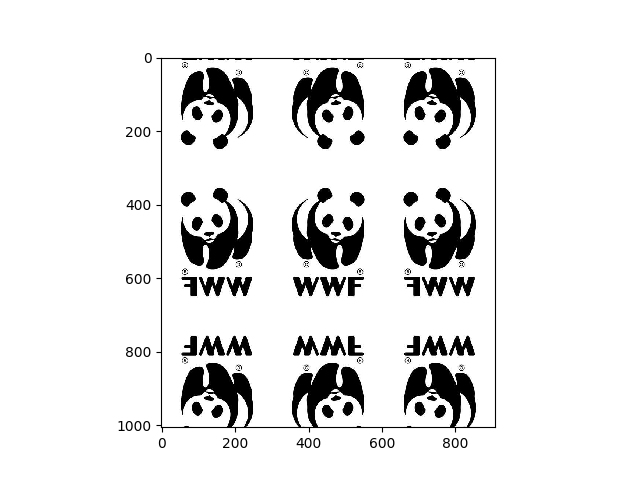
\includegraphics[scale=0.8]{WWF_bord}
	\end{center}

	De plus, l'idée étant de rendre plus lisse des images bruitées, nous avons écrit un algorithme qui va bruiter nos images : \emph{\textbf{bruit.py}}
	
	%\lstinputlisting[language = Python]{bruit.py}
	
	Ainsi, pour la suite, nous allons brouiller \textsc{Ted} et travailler sur l'image suivante : 
	
	\begin{center}
		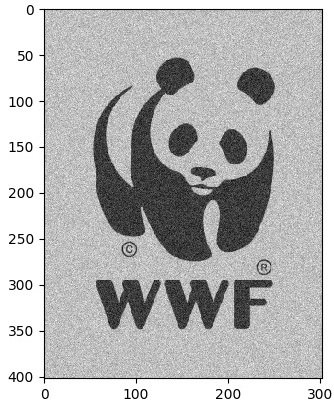
\includegraphics[scale=0.8]{WWF_bruit}
	\end{center}
	
		
	\chapter*{En Dimension 1}
	
	\section*{Problème Linéaire 1D}
	
	Dans cette section, nous allons discrétiser le problème de l'équation de la chaleur linéaire qui est le suivant : 
	
	\begin{equation}
	\left\{
	\begin{aligned}
	&\frac{\partial u}{\partial t}=\Delta u(t,x) &\qquad &\text{ sur } \Omega \\
	&\frac{\partial u}{\partial N} = 0 &\qquad &\text{ sur } \partial \Omega \times \left(0,T\right) \\
	&u(0,x) = u_0(x) &\qquad &\text{ dans } \Omega
	\end{aligned}
	\right.
	\end{equation}
	
	Pour cela, il nous faut, grâce à nos calculs préliminaires, discrétiser le \textbf{Laplacien}, qui correspond, dans le cas 1D, à l'approximation de la dérivée seconde. Pour cela on fait la combinaison linéaire suivante à partir des formules de Taylor : \ref{eq1}+\ref{eq2}. On obtient 
	\[
	\Delta u_i = u_{i+1}-2u_{i}+u_{i-1}
	\]
	
	On en conclut alors la forme discrétisée de notre équation de la chaleur en dimension 1 
	\[
	u^{n+1}_{i} = u^{n}_{i} + \delta t(u^{n}_{i+1}-2u^{n}_{i}+u^{n}_{i-1})
	\]
	
	Grâce à cette formule, nous avons écrit le code \emph{\textbf{problemelin1D.py}} pour le cas 1D dans lequel nous avons introduit notre condition de $CFL$, calculée en fonction du pas de temps $\delta t$.
	
	%\lstinputlisting[language = Python]{problemelin1D.py}
	
	
	\section*{Perona-Malik 1D}
	
	Pour améliorer les résultats obtenus par l'équation de la chaleur, Perona et Malik ont proposé de modifier l'équation en y intégrant le processus de détection des bords. Ce modèle permet de lisser les régions homogènes en préservant les bords. On rappelle l'équation de la chaleur \textbf{non-linéaire} :
	
\begin{equation*}
\left\{
\begin{aligned}
&\frac{\partial u}{\partial t} = \div\left(c\left(\left|\nabla u\right|\right)\nabla u\right) &\qquad &\text{ sur } \Omega \\
&\frac{\partial u}{\partial N} = 0 &\qquad &\text{ sur } \partial \Omega \times \left(0,T\right) \\
&u(0,x) = u_0(x) &\qquad &\text{ dans } \Omega 
\end{aligned}
\right.
\end{equation*}

	où $\left|\nabla u\right|$ est la norme du gradient de $u$ et $c$ est une fonction décroissante de $\R^+$ dans $\R^+$. 
	
	Dans notre cas, nous utiliserons 
	\[
	c(t) = \displaystyle\frac{1}{1+\left(\frac{t}{\alpha}\right)^2}	
	\]
	
	En dimension 1, la norme du gradient n'est autre que la discrétisation du gradient (avec une racine carrée qui sera supprimée par le terme au carré dans la fonction $c$), nous n'avons donc pas de calculs particuliers à faire. 
	
	On utilise toujours un schéma d'\textbf{Euler explicite}
	
	\begin{equation*}
	\frac{\partial u}{\partial t}=\frac{u^{n+1}_{i}-u^{n}_{i}}{\delta t}.
	\end{equation*}
	
	Et on obtient pour la discrétisation de l'espace en utilisant des différences finies décentrées à droite
	\[
	c_{i}\nabla_{i} = c_i\left(u_{i+1} - u{i}\right) - c_{i-1}\left(u_i - u_{i-1}\right)
	\]
	
	On peut finalement écrire la discrétisation générale : 
	\[
	u^{n+1}_i = u^n_i + \delta t\left(c_i\left(u^n_{i+1} - u^n{i}\right) - c_{i-1}\left(u^n_i - u^n_{i-1}\right)\right)
	\]
	
	Nous avons alors écrit un premier fichier Python contenant la discrétisation du gradient ainsi que la fonction $c$ que nous utilisons : \emph{\textbf{C1D.py}}.
	
	%\lstinputlisting[language = Python]{C1D.py}
	
	Enfin, nous avons codé le procédé de Perona-Malik dans le cas de la dimension 1 dans le fichier \emph{\textbf{Perona1D.py}}
	
	%\lstinputlisting[language = Python]{Perona1D.py}
	
	
	
	\chapter*{En Dimension 2}
	
	\section*{Problème Linéaire 2D}
	
	On rappelle le problème de l'équation de la chaleur linéaire 
	
	\begin{equation}
	\left\{
	\begin{aligned}
	&\frac{\partial u}{\partial t}=\Delta u(t,x) &\qquad &\text{ sur } \Omega \\
	&\frac{\partial u}{\partial N} = 0 &\qquad &\text{ sur } \partial \Omega \times \left(0,T\right) \\
	&u(0,x) = u_0(x) &\qquad &\text{ dans } \Omega
	\end{aligned}
	\right.
	\end{equation}
	
	Dans cette section, nous allons discrétiser le problème de l'équation de la chaleur dans le cas 2D. Nous allons commencer, comme dans l'exemple précédent, par discrétiser le \textbf{Laplacien}. On obtient alors 
	
	\begin{align*}
	\Delta u_{i,j}
	& =  \frac{\partial}{\partial x_1}(u_{i+1,j}-u_{i,j})+\frac{\partial}{\partial x_2}(u_{i,j+1}-u_{i,j}) \\
	& =  u_{i+1,j}-u_{i,j}-(u_{i,j}-u_{i-1,j}) + u_{i,j+1}-u_{i,j}-(u_{i,j}-u_{i,j-1})  \\
	& =  u_{i+1,j}-2u_{i,j}+u_{i-1,j} + u_{i,j+1}-2u_{i,j}+u_{i,j-1} \\
	& =  u_{i+1,j}+u_{i-1,j}+u_{i,j+1}+u_{i,j-1}-4u_{i,j}.
	\end{align*}
	
	On en déduit alors la discrétisation du problème 
	\[
	u^{n+1}_{i,j} = u^{n}_{i,j} + \delta t(u^{n}_{i+1,j}+u^{n}_{i-1,j}+u^{n}_{i,j+1}+u^{n}_{i,j-1}-4u^{n}_{i,j})
	\]
	
	De cette formule, on écrit l'algorithme \emph{\textbf{problemelin2D.py}}

	%\lstinputlisting[language = Python]{problemelin2D.py}
	
	Voici le résultat obtenu pour une valeur de $\delta t = 0.1$, et $35$ itérations. L'image de gauche représente l'image brouillée, celle de droite l'image après le traitement par l'équation de la chaleur linéaire.
	
	\begin{figure}[htbp]
    \centering
    \begin{subfigure}[b]{0.45\textwidth}
        \centering 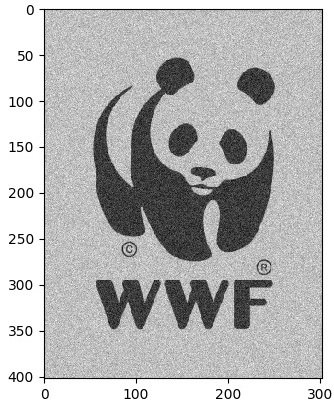
\includegraphics[width=\textwidth]{WWF_bruit}
        \caption{TED bruité}
    \end{subfigure}
    ~
    \begin{subfigure}[b]{0.45\textwidth}
        \centering 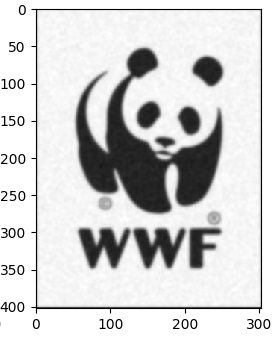
\includegraphics[width=\textwidth]{TED_chaleur.png}
        \caption{TED filtré par l'EDP de la chaleur}
    \end{subfigure}
    \caption{}
	\end{figure}

	
	\section*{Perona-Malik 2D}
	
	On rappelle l'équation de la chaleur \emph{non-linéaire} dans le cas de \textsc{Perona-Malik}
	
	\begin{equation*}
	\left\{
	\begin{aligned}
	&\frac{\partial u}{\partial t} = \div\left(c\left(\left|\nabla u\right|\right)\nabla u\right) &\qquad &\text{ sur } \Omega \\
	&\frac{\partial u}{\partial N} = 0 &\qquad &\text{ sur } \partial \Omega \times \left(0,T\right) \\
	&u(0,x) = u_0(x) &\qquad &\text{ dans } \Omega 
	\end{aligned}
	\right.
	\end{equation*}
	
	où $\left|\nabla u\right|$ est la norme du gradient de $u$ et $c$ est une fonction décroissante de $\R^+$ dans $\R^+$. 
	
	Dans notre cas, nous utiliserons 
	\[
	c(t) = \displaystyle\frac{1}{1+\left(\frac{t}{\alpha}\right)^2}	
	\]

	Comme précédemment, nous obtenons par \textbf{Euler explicite}
	
	\begin{equation*}
	\frac{\partial u}{\partial t}=\frac{u^{n+1}_{i,j}-u^{n}_{i,j}}{\delta t}.
	\end{equation*}
	
	On commence par discrétiser la norme du gradient en utilisant des différences finies décentrées à droite
	 
	\begin{equation*}
	c_{i,j} = c\left(\left|\nabla u_{i,j}\right|\right) = c\left(\sqrt{(u_{i+1,j}-u_{i,j})^2 +(u_{i,j+1} -u_{i,j})^2}\right)
	\end{equation*}
	
	On discrétise ensuite
	
	\begin{equation*}
	c_{i,j}\nabla u_{i,j} = c_{i,j}\left(u_{i+1,j}-u_{i,j} \quad ;\quad u_{i,j+1}-u_{i,j}\right)
	\end{equation*}
	
	On sait que, si l'on utilise une discrétisation décentrée à droite du gradient, on peut exprimer la divergence de la façon suivante
	\[
	\left(\div\left(p\right)\right)_{i,j} = p^1_{i,j} - p^1_{i-1,j} + p^2_{i,j} - p^2_{i,j-1}
	\]
	
	En reprenant nos calculs on obtient alors pour la divergence 	
	\begin{equation*}
	\div\left(c_{i,j}\nabla u_{i,j}\right) =  c_{i,j}\left(u_{i+1,j}-u_{i,j}\right)-c_{i-1,j}\left(u_{i,j}-u_{i-1,j}\right)+c_{i,j}\left(u_{i,j+1}-u_{i,j}\right)-c_{i,j-1}\left(u_{i,j}-u_{i,j-1}\right)
	\end{equation*}
	
	Sachant que,	
	
	\begin{equation*}
	u_{i,j}^{n+1} = u_{i,j}^{n} + \delta t\div\left(c_{i,j}^{n}\nabla u_{i,j}^{n}\right)
	\end{equation*}
	
	On obtient finalement,
	
	\begin{equation*}
	u_{i,j}^{n+1} = u_{i,j}^{n} + \delta t \left( c_{i,j}\left(u^n_{i+1,j}-u^n_{i,j}\right)-c_{i-1,j}\left(u^n_{i,j}-u^n_{i-1,j}\right)+c_{i,j}\left(u^n_{i,j+1}-u^n_{i,j}\right)-c_{i,j-1}\left(u^n_{i,j}-u^n_{i,j-1}\right) \right)
	\end{equation*}
	
	Pour l'écriture algorithmique, nous avons d'abord écrit un fichier comprenant la discrétisation du gradient ainsi que la fonction $c$ que nous utilisons : \emph{\textbf{C2D.py}}
	
	%\lstinputlisting[language = Python]{C2D.py}
	
	Puis nous avons finalement écrit l'algorithme pour Perona-Malik en reprenant les mêmes techniques que précédemment : \emph{\textbf{Perona2D.py}}
	
	%\lstinputlisting[language = Python]{Perona2D.py}
	
	Voici le résultat obtenu pour un pas de temps $\delta t = 0.1$, $35$ itérations et une valeur de $\alpha = 1000$.
	
	\begin{figure}[htbp]
    \centering
    \begin{subfigure}[b]{0.45\textwidth}
        \centering 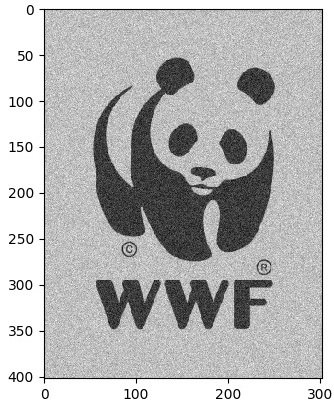
\includegraphics[width=\textwidth]{WWF_bruit}
        \caption{TED bruité}
    \end{subfigure}
    ~
    \begin{subfigure}[b]{0.45\textwidth}
        \centering 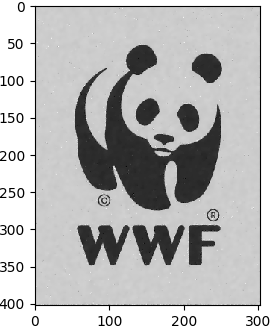
\includegraphics[width=\textwidth]{TED_perona}
        \caption{TED filtré par Perona-Malik}
    \end{subfigure}
    \caption{}
	\end{figure}
	
	\begin{figure}[htbp]
    \centering
    \begin{subfigure}[b]{0.45\textwidth}
        \centering \includegraphics[width=\textwidth]{cameraman_chaleur2D}
        \caption{Chaleur : 0.1/50}
    \end{subfigure}
    ~
    \begin{subfigure}[b]{0.45\textwidth}
        \centering \includegraphics[width=\textwidth]{cameraman_perona2D}
        \caption{Perona-Malik : 0.1/50/1000}
    \end{subfigure}
	
    \begin{subfigure}[b]{0.46\textwidth}
        \centering \includegraphics[width=\textwidth]{lenna_chaleur2D}
        \caption{Chaleur : 0.1/35}
    \end{subfigure}
    ~
    \begin{subfigure}[b]{0.45\textwidth}
        \centering \includegraphics[width=\textwidth]{lenna_perona2D}
        \caption{Perona-Malik : 0.1/35/1000}
    \end{subfigure}
    \caption{Différence entre l'EDP de la chaleur et Perona-Malik}
	\end{figure}


	
	
\end{document}
